\documentclass[varwidth]{standalone}

\usepackage{tikz}
\usetikzlibrary{shapes.geometric, arrows, calc, positioning}

\tikzstyle{morning} = [rectangle, rounded corners, minimum width=3cm, minimum
height=2cm,text centered, text width = 3cm, draw=black, fill=green!30]

\tikzstyle{afternoon} = [rectangle, rounded corners, minimum width=3cm, minimum
height=2cm,text centered, text width = 3cm, draw=black, fill=red!30]

\tikzstyle{evening} = [rectangle, rounded corners, minimum width=3cm, minimum
height=2cm,text centered, text width = 3cm, draw=black, fill=blue!30]


\tikzstyle{arrow} = [thick,->,>=stealth]

\usepackage{graphicx}


\title{Timetable(Version 1)}
\author{Wenkai Wu}

\begin{document}
\maketitle{}


\includegraphics[height=3em]{writing.png}

\includegraphics[height=3em]{graduation.png}

\begin{figure}
  \centering


    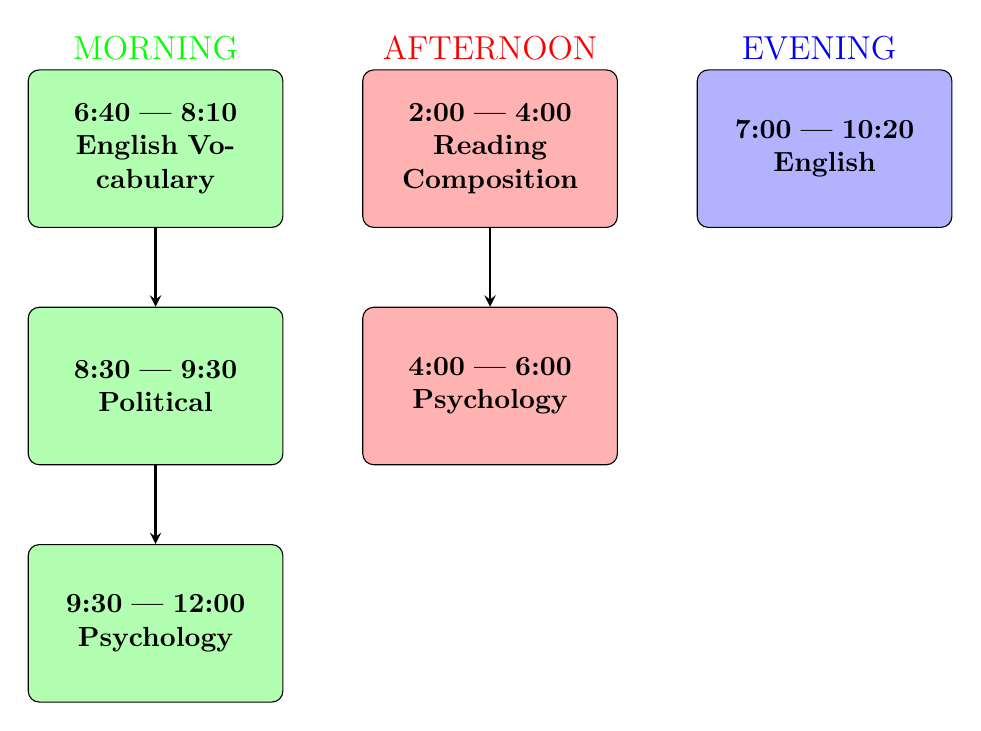
\begin{tikzpicture}
      \node (mor2) [morning, label=above: {\large \color{green} MORNING}] {\bf 6:40 — 8:10
        \\ English Vocabulary};
      \node (mor3) [morning, below=of mor2] {\bf 8:30 — 9:30 \\ Political};
      \node (add1) [morning, below=of mor3] {\bf 9:30 — 12:00 \\ Psychology};

      \node (aft2) [afternoon, right=of mor2, label=above: {\large \color{red} AFTERNOON}]
      {\bf 2:00 — 4:00 \\ Reading \\ Composition};
      \node (aft3) [afternoon, below=of aft2] {\bf 4:00 — 6:00 \\ Psychology};

      \node (eve1) [evening, right=of aft2, label=above: {\large \color{blue} EVENING }] {\bf 7:00 — 10:20 \\ English};

      \draw [arrow] (mor3) -- (add1);
      \draw [arrow] (mor2) -- (mor3);
      \draw [arrow] (aft2) -- (aft3);
    \end{tikzpicture}
  

  % \textcolor{red}{Fighting}

\end{figure}

\includegraphics[height=3em]{trophy.png}
\dotfill

\includegraphics[height=3em]{biking.png}

% \textcolor{red}{Fighting}

\end{document}



%%% Local Variables:
%%% mode: latex
%%% TeX-master: t
%%% End:
